% !TEX root = SocialVision2012.tex
\pagestyle{plain} \pagenumbering{arabic}

\Section{Introduction} \label{sec:intro}

%The past decade has produced stunning advances in computer vision. Real-time face detection that was introduced at the turn of the millennium is now commonplace in personal electronic devices. Face recognition has evolved from just a research topic to a widely-used tool for managing photo collections. Built on academic research from the 1990's, we now have systems like Microsoft Photosynth and Google Earth that can automatically reconstruct three-dimensional models from large, unstructured photo collections. And thanks to the growing availability of annotated image collections and research in vision and machine learning, our ability to distinguish between object categories has improved dramatically, enabling applications from image search to product identification. If the purpose of computer vision is to extract from image data useful information about the world, it is clear that we now have useful, functioning vision systems for more than a few types of information. 


The past decade has produced stunning advances in computer vision. Real-time face detection introduced at the turn of the millennium is now commonplace in personal electronics. Face recognition has evolved from a research topic to a widely-used tool for managing photo albums. We now also have systems like Microsoft Photosynth and Google Earth that can automatically reconstruct 3D models, and our ability to distinguish between object categories has improved dramatically, enabling applications from image search to product identification. If the mission of computer vision is to extract from imagery useful information about the world, it is clear that we now have functioning systems for more than a few types of information. 


%Yet, there are aspects of the world to which computer vision systems remain quite blind. Prominent among these are \emph{social interactions} and \emph{social relationships} between people. This information will undoubtedly be useful for machines, just as it is useful for humans when recognizing individuals within a social group from large distances; when making decisions about which colleagues to approach to enact policy changes; or when deciding whether or not to alert authorities about a questionable interaction between strangers.

Yet, there are aspects of the world to which computer vision remains quite blind. Prominent among these are \emph{social interactions} and \emph{social relationships} between people. This information is undoubtedly useful for machines, just as it is useful for humans when analyzing individuals within a social group from a distance; when deciding which colleagues to approach to enact policy changes; or when judging whether to alert authorities of a questionable interaction between strangers.


%We propose to develop foundations for computer vision systems that are `socially aware', in the sense of being able to recover social information from imagery. These systems will extract, from images and videos of human gatherings,  information about the types and frequencies of social interactions that occur within these gatherings, and from this they will compute useful information about the social network that embeds the observed individuals, groups, and communities.  Our work will introduce computer vision as a new source of social network information, one that complements email logs, phone logs, web-based community connections, and so on. Vision is an important complement to these because it provides access to relative face positions, body positions, movements, gestures, and expressions, all of which are difficult to observe by any other means, and all of which are critical signals for analyzing interactions and relationships between people. 


We propose to develop foundations for computer vision systems that are `socially aware', in the sense of being able to recover social information from imagery. These systems will extract, from images and videos of human gatherings,  information about the types and frequencies of social interactions that occur, and compute useful information about the social network that embeds the individuals, groups, and communities.  Our work will introduce computer vision as a new source of social network information, one that complements emails, phone logs, web-based community connections, and so on. Vision is an important complement to them, because it provides access to face positions, body poses, gestures, and expressions, and scenes, all of which are difficult to observe by any other means, but are critical signals for analyzing interactions and relationships. 

%Our research is timely because of the recent maturation of technologies for detecting and tracking the faces and bodies of individual people and recognizing their identities. A variety of practical systems currently exist for face detection and person detection, and by integrating these with tracking techniques in monocular systems or camera arrays, these can yield crude but useful descriptors of individual behaviors in the form of positions, velocities, histograms-of-flow, bags of space-time interest points, and so on. When resolution and image quality permits, these can also be augmented with more detailed per-individual descriptors computed from head pose, facial expression, and body pose. In any case, with environment-appropriate detection and tracking, along with the extraction of suitable descriptors for the detected and tracked individuals, an image or video can be abstracted as a collection of (fragmented and noisy) individual trajectories with accompanying (time-varying) behavior descriptors (see ${\bf f}$ for still image and ${\bf f}(t)$ for video in Fig.~\ref{fig:intro}). And this is the abstraction on which our proposed methods will operate.


Our research is timely because of the recent maturation of technologies for detecting and tracking the faces and bodies of people and recognizing their identities. A variety of practical systems currently exist, and an appropriate integration of them can yield crude but useful descriptors of individual behaviors in the form of trajectories, histograms-of-flow, bags of interest points, and so on. When image quality permits, these can also be augmented with more detailed per-individual descriptors computed from head pose, facial expression, and body pose. In any case, with these descriptors an image or video can be abstracted as a collection of (fragmented and noisy) individual trajectories with accompanying (time-varying) behavior descriptors (see ${\bf f}$ for still image and ${\bf f}(t)$ for video in Fig.~\ref{fig:intro}). And this is the abstraction on which our proposed methods will operate.

\begin{figure}[t!]
\begin{center}
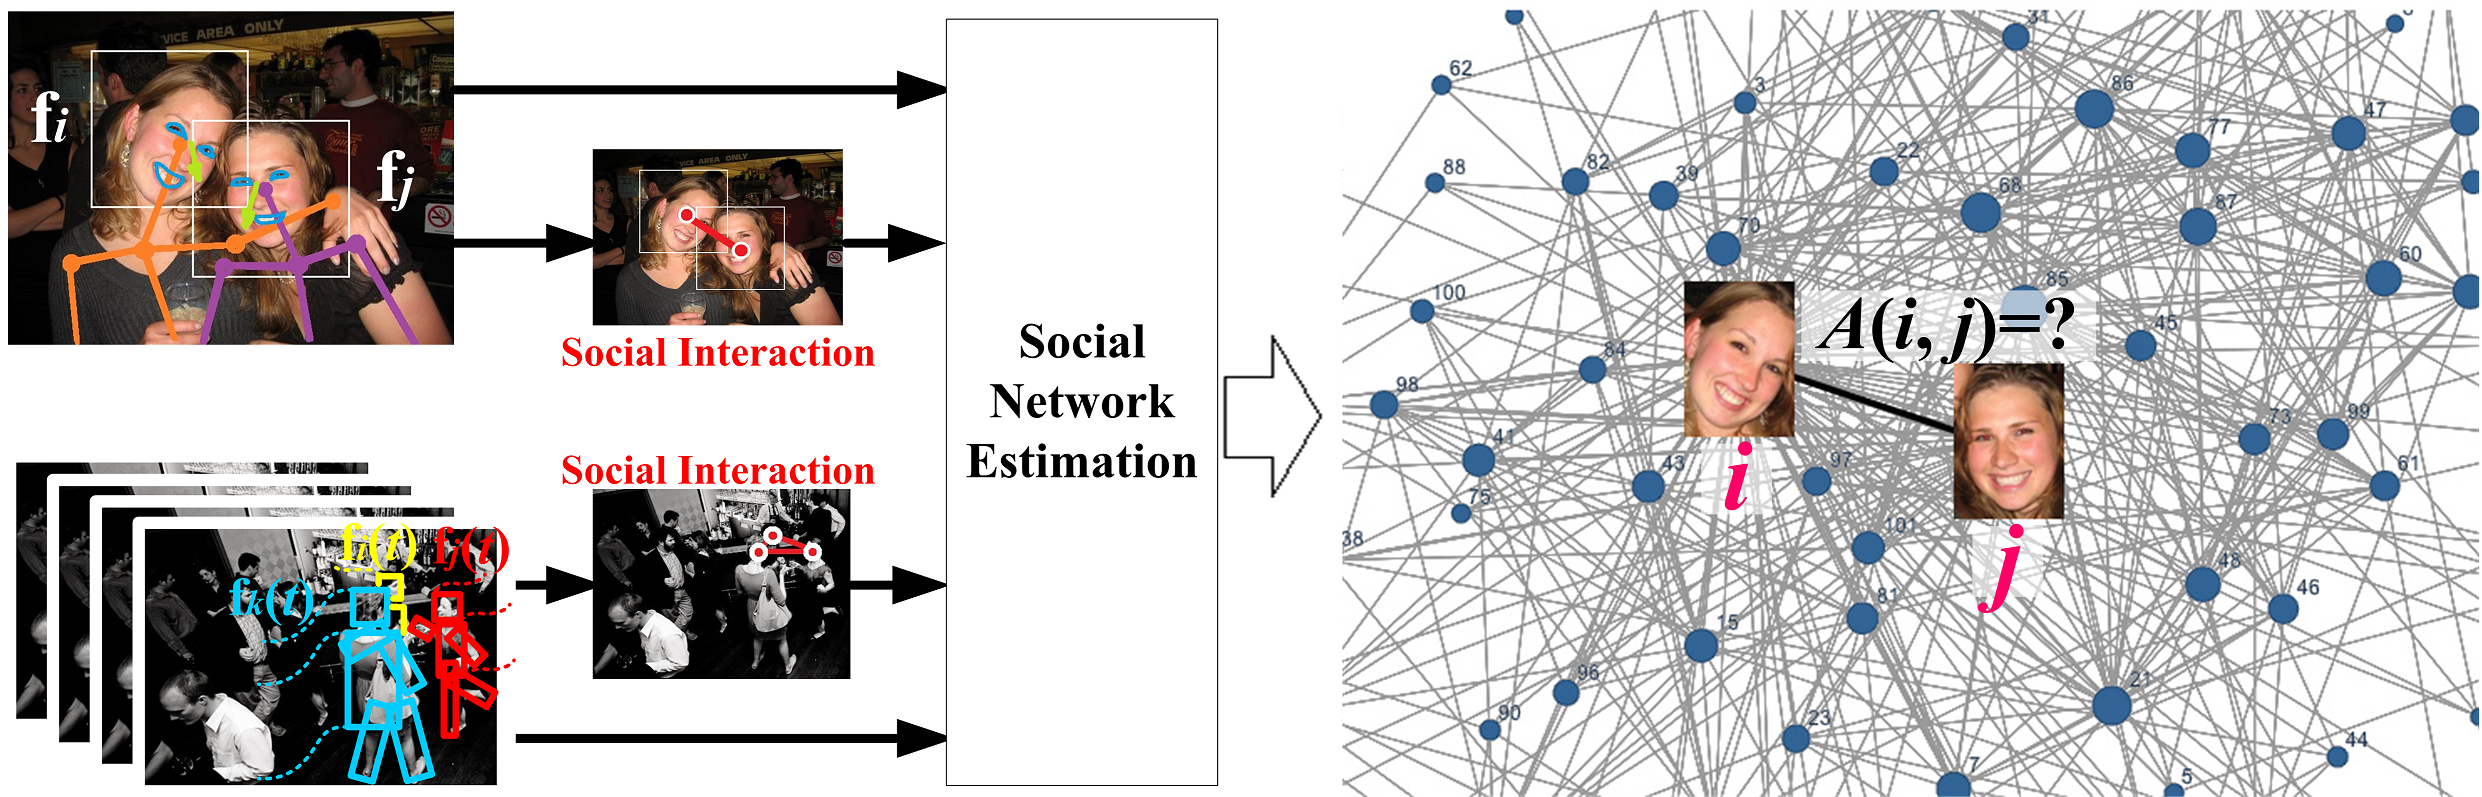
\includegraphics[width=\columnwidth]{intro_1}
\end{center}
\vspace{-0.25in} \caption{\captionsize 
Social visual analytics: A computer vision approach to `sense' a social network. \label{fig:intro}\afterfigspace}
\end{figure}

Our project can be described in four parts:

\begin{enumerate}

\item Representing, detecting, and recognizing social interactions. Broadly speaking, we consider a social interaction to be a co-occurrence of two or more individual behaviors that are together distinctive in space and time. Based on this definition, we will develop new representations of social interactions comprised of mixed ensembles of individual behavior descriptors and relative pair-wise behavior descriptors, inspired by computational sociology~\cite{Kendon1990,Lazer2009,Pantic}. With them we will develop methods for detecting and recognizing occurrences of pre-defined interaction categories in large social gatherings, and preliminary results show that they provide an attractive balance of discriminative power, robustness, and efficiency.

\item Learning new categories and optimal detectors for social interactions. Sociology suggests that social interactions can often be usefully categorized into a manageable number of classes (e.g.,~\cite{Kendon1990,Hoyle,Tannen,econo_category,Scherr2009}), but discovering these categories is currently an onerous task for human experts that cannot be easily scaled to many different environments or to situations involving more than a few participants. To address this, we will develop computational tools for supervised and semi-supervised learning of interaction categories. Once we have obtained socially-meaningful interaction categories, we learn effective and efficient detectors for them.

\item Inferring social networks from observed interactions. We will create computational methods for estimating a social network from multiple visual cues including detected occurrences of social interactions. We argue that existing tools for reconstructing social networks from sensor measurements are not optimized to work for vision, and we propose a new class of techniques to improve performance when: (a) the visual descriptors are derived from diverse sources, very noisy, and even missing; (b) the underlying social network is described in multiple-views; and (c) the identities associated to image targets are ambiguous. 

\item Data collection and challenge problems. We will collect datasets to evaluate our methods and design challenge problems to engage our colleagues in this research agenda. To do this, we will address the challenge of enabling reproducible research while preserving privacy.

\end{enumerate}

%Our goal is to enable the automatic recovery of useful information about social interactions and the underlying social network using \emph{today's} technology for identity recognition and face and body detection and tracking, with the understanding that our accuracy will automatically increase as face and body analysis tools continue to evolve. A principal challenge we address, therefore is how to handle the substantial and unavoidable uncertainties caused by false detections, broken tracks, and mis-recognitions. We also seek general methods that can exploit inputs of varying precision.  High-quality videos from a meeting can provide fine-scale information about pose and expression, while low-quality surveillance video might provide only coarse estimates of head pose. Our goal is to create general tools that operate in both of these cases and more, automatically making use of as much facial information as is available.

Our goal is to enable the automatic recovery of useful information about social interactions and the underlying social network using \emph{today's} tools, with the understanding that our accuracy will automatically increase as these tools continue to evolve. A principal challenge, therefore is to handle the substantial and unavoidable uncertainties caused by false detections, broken tracks, and mis-recognitions, and we seek general methods that can exploit inputs of varying precision. High-quality videos can provide fine-scale information about expression, while low-quality surveillance might provide only coarse estimates of head pose. Our goal is to create general tools that operate in all cases and make use of as much information as is available.


%The proposed research will provide a foundation for socially-aware computer vision systems. These systems will transform security, anti-terrorism, autonomous visual analytics, augmented reality, human computer interaction, human resource planning, operations research, game theory and e-commerce, and identify recognition. The research will be carried out by a team with established expertise in recognition of identities, activities, and interactions, as well as collecting and analyzing social image and video collections. PI Todd Zickler has pioneered research on the use of social network context to improve identity recognition~\cite{Stone2008,Stone2010} and led the implementation of a camera-based system for long-term observation of social interactions in an interactive classrooms (Section~\ref{sec:sys}). PI Ruonan Li has substantial expertise in group interactions recognition~\cite{LiIJCV2012}, analyzing human activities and behaviors~\cite{Li2010,LiPAMI2012}, and domain adaptation methods for learning appearance models when annotated training data is difficult or expensive to acquire~\cite{LiZickler2012,Li2011}. 

The proposed research will provide a foundation for socially-aware computer vision systems that will transform security, autonomous scene analytics, augmented reality, human computer interaction, human resource planning, operations research, and e-commerce. The research will be carried out by a team with established expertise in recognition of identities, activities, and interactions, as well as collecting and analyzing social image and video collections. PI Todd Zickler has pioneered research on the use of social network context to improve recognition~\cite{Stone2008,Stone2010} and led the implementation of a camera-based system for long-term observation of social interactions (Section~\ref{sec:sys}). PI Ruonan Li has substantial expertise in activity recognition~\cite{LiIJCV2012}, analyzing human behaviors~\cite{Li2010,LiPAMI2012}, and adapting existing models when annotated training data is difficult or expensive to acquire~\cite{LiZickler2012,Li2011}. 

%The proposal is organized as follows. Following a discussion of related work in Section 2, we being our proposed research in Section 3.1 by discussing representations for social interactions and the detection and recognition of an interaction in an image or a long video of a large social gathering. In Section 3.2, we discuss how this technology will  discover and learn salient interaction categories in semi-supervised and unsupervised scenarios, and ho wit will optimize the detection and recognition. Section 3.3 moves on to describe how to infer social network information from interactions that are detected over time and space in large image and video collections, with a focus on robustly associating identities to targets in the images/videos and effectively reconstructing noisy and incomplete multi-view networks. Finally, Section 3.4 describes data collection and challenge problems for evaluation.



%%%%%%%%%%%%%%%%%%%%%%%%%%%%%%%%%%%%%%%%%

%\begin{enumerate}
%\item  Detecting and recognition of interaction categories. Relatively mature in images due to face detection, person detection, and pose estimation.  But largely unsolved in videos. We will address the questions including 1) How do we represent an interaction category? 2) How do we identify in a long video of a large gathering 3) when this interaction occurs, and 4) who it involves? To do so, we will develop approaches to learn effective and efficient interaction detector for  a given set of categories. These socially-salient interaction categories may arise from sociology \cite{Kendon1990,Ekman,Hoyle,Tannen,Goodwin2000,Goldin,Goodwin2007,Kendon2010,Lazer2009}, but this does not scale in novel environments and applications. Therefore, we will develop approaches to learn representations for new categories from image/video collections in a semi-supervised or unsupervised manner.
%\item Inferring social network information from detected interactions. We will design mechanisms by which we distill ties or affinities between social members from multiple heterogeneous visual cues, and in particular accounting for the multi-view effect in a practical social network. To achieve robustness, our research will especially focus on noise-resilient methods for mapping image targets to the identities of the members, as well as novel algorithms to the case of incomplete and noisy outputs from the social network estimator due to various types of imperfection incurred from missed detections; mis-classified interactions, and a large fraction of missing observations.
%\item Data collections and challenge problems. We will collect datasets to evaluate our methods and design challenge problems to engage our colleagues in this research agenda. To do this, we will address the challenges of enabling reproducible research while preserving privacy.
%\end{enumerate}


